\chapter{Examples} \label{chap:examples}
The pruning algorithm is presented on several examples, where each of them has its purpose of being shown. The XOR problem (\cref{sec:dataset_xor}) should verify the ability of finding an optimal network structure. Section \ref{sec:dataset_unbfea} comes with another 2D problem, where one feature carries more information than the other one. The Rule-plus-Exception problem in \cref{sec:dataset_rpe} deals with a minority of samples that has to be treated by a different net part than rule-based samples. The train problem (\cref{sec:dataset_train}) is a working example of feature selection procedure. The MNIST database (\cref{sec:dataset_mnist}) is widely used in machine learning and can be regarded as commonly known. Therefore it is a good example for presentation of new methods. Finally, in \cref{sec:dataset_phonemes} the pruning algorithm is applied on a large dataset of phonemes.

\section{2D-problem A: XOR Function} \label{sec:dataset_xor}
The standard Exclusive OR (XOR) function is defined by truth \cref{tab:examples:xor_function}. Based on this function one can build a classification problem with two features and two classes.

\begin{table}[H]
\centering
\begin{tabular}{|c|c||c|}
\hline
\textit{$ x_1 $} & \textit{$ x_2 $} & \textit{y} \\ \hline \hline
0                & 0                & 0          \\ \hline
0                & 1                & 1          \\ \hline
1                & 0                & 1          \\ \hline
1                & 1                & 0          \\ \hline
\end{tabular}
\caption{Standard XOR function.}
\label{tab:examples:xor_function}
\end{table}

This problem serves perfectly for demonstration of network optimization methods, as two optimal architectural solutions producing the XOR function are known (\cref{fig:examples:xor_solutions}) \footnote{The known (e.g. from \citep{online:xor_solution}) minimal network architectures producing the XOR function $ [2, 2, 1] $ and $ [2, 3, 1] $ are adjusted to $ [2, 2, 2] $ and $ [2, 3, 2] $ in \cref{fig:examples:xor_solutions} in order to comply with the conventions introduced in \cref{chap:methods}. The number of output neurons always equals the number of classes. The number of synapses connected to the output layer is a subject to think about.}. 

\begin{figure}[H]
\centering
\begin{subfigure}{.4\textwidth}
  \centering
  \includegraphics[height=2cm]{xor_min1}
  \caption{Solution A.}
  \label{fig:examples:xor_min1}
\end{subfigure}
\begin{subfigure}{.4\textwidth}
  \centering
  \includegraphics[height=2cm]{xor_min2}
  \caption{Solution B.}
  \label{fig:examples:xor_min2}
\end{subfigure}
\caption{Optimal network architectures producing the XOR function.}
\label{fig:examples:xor_solutions}
\end{figure}

With this knowledge we can prove that the pruning algorithm is (or is not) able to find the optimal solution. If the method is correct, it should end up with one of the shown architectures (\cref{fig:examples:xor_min1} or \cref{fig:examples:xor_min2}).

The truth \cref{tab:examples:xor_function} ruled the generation of a 2D dataset illustrated in \cref{fig:examples:dataset_xor}. The two classes can be linearly separated by two lines (two neurons, see \cref{fig:examples:xor_min1}) and each class consists of 1000 samples. Each sample was randomly assigned to one of the two possible points belonging to its class (e.g. (0,0) or (1,1) for class 0) and then randomly placed in the surounding area within a specified range ($ r = \frac{\sqrt{2}}{4} $).

The samples of each class were then splitted into three sets in the following manner: $ 80\% $ to a training set, $ 10\% $ to a validation set and $ 10\% $ to a testing set.

\begin{figure}[H]
\centering
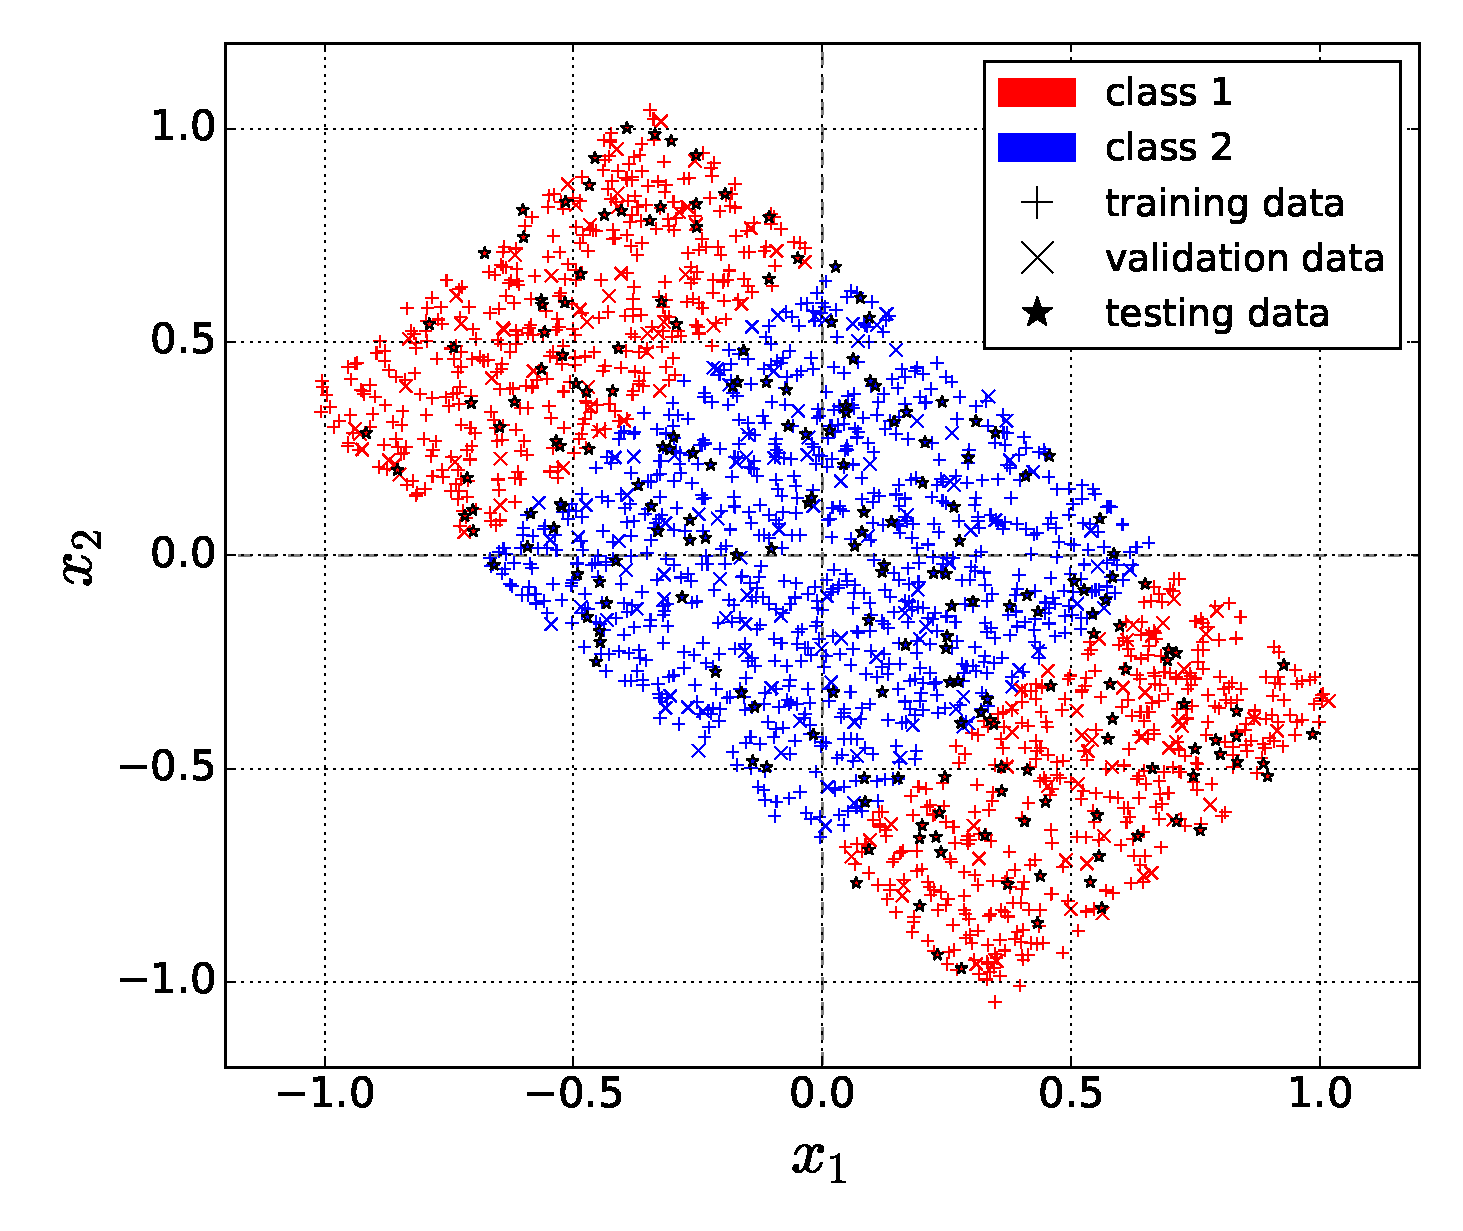
\includegraphics[width=0.9\textwidth]{dataset_xor.eps}
\caption{The XOR dataset.}
\label{fig:examples:dataset_xor}
\end{figure}

The goal of this example is to show that the pruning algorithm finds one of the known minimal network structures (\cref{fig:examples:xor_solutions}). An oversized network $ [2, 50, 2] $ is used as the starting point. The following \cref{tab:examples:xor_settings} shows all the experiment settings.

\begin{table}[H]
\centering
\scalebox{0.95}{
\begin{tabular}{|l|c|l|c|l|c|}
\hline
\multicolumn{2}{|c|}{\textit{initial network}} & \multicolumn{2}{c|}{\textit{learning parameters}} & \multicolumn{2}{c|}{\textit{pruning parameters}} \\ \hline
structure             & {[}2, 50, 2{]}         & learning rate                  & 0.3              & required accuracy             & 1.0              \\ \hline
transfer fcn          & sigmoid                & number of epochs               & 50               & retrain                       & True             \\ \hline
                      &                        & minibatch size                 & 1                & retraining epochs             & 50               \\ \hline
\end{tabular}}
\caption{Experiment settings for XOR dataset.}
\label{tab:examples:xor_settings}
\end{table}

\subsection*{Results: XOR Function}
\cref{fig:examples:pruning_process_xor} describes the pruning process. We can see the number of synapses (starting with $ 200 $ for fully-connected structure $ [2, 50, 2] $), the network structure and classification accuracy at single pruning steps (see [PA]). When the required accuracy ($ 1.0 $) was not reached, the corresponding steps are transparent in the figure, indicating they were forgotten.

\begin{figure}[H]
\centering
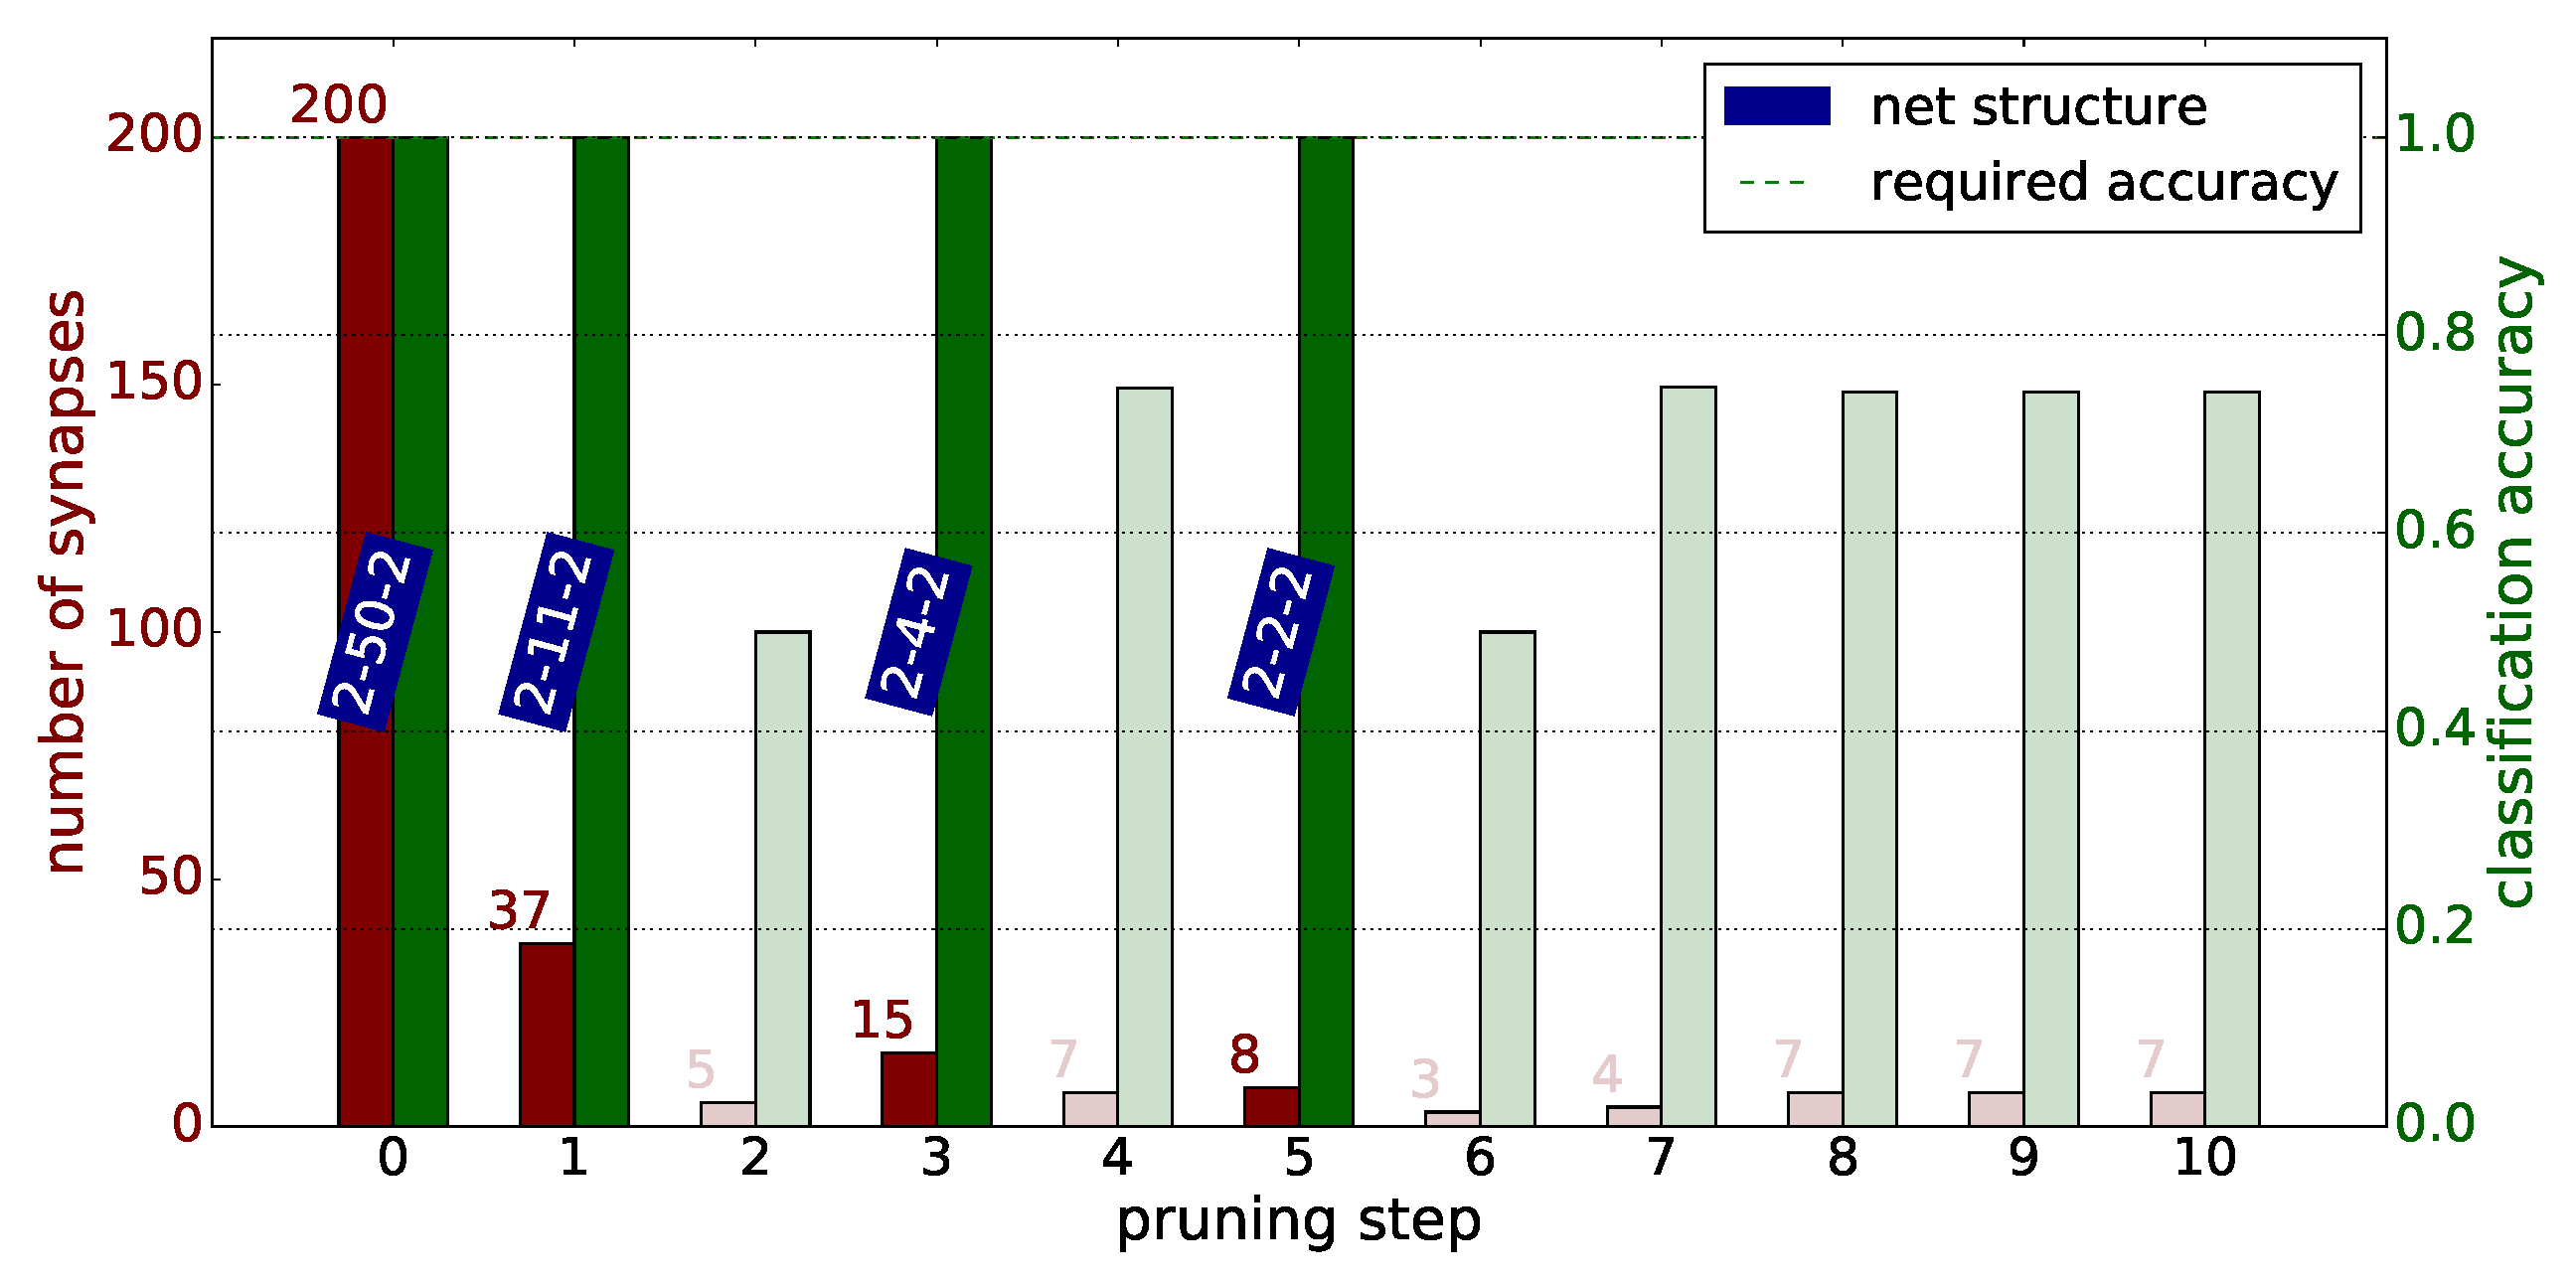
\includegraphics[width=\textwidth]{pruning_process_xor.eps}
\caption{Illustration of the pruning procedure applied on XOR dataset (selected observation).}
\label{fig:examples:pruning_process_xor}
\end{figure}

In \cref{fig:examples:pruning_result_xor} the hypothesis of this experiment is confirmed. In \cref{fig:examples:pie_xor} we can see that in $ 47 $ out of $ 100 $ cases the pruning algorithm changed the network to $ [2, 2, 2] $ architecture (\cref{fig:examples:xor_min1}), in $ 45\% $ of the cases it resulted with $ [2, 3, 2] $ (\cref{fig:examples:xor_min2}) and only in $ 8\% $ it failed to find the optimal architecture. \cref{fig:examples:result_synapses_xor} gives statistics for the final number of synapses in these three cases.

\begin{figure}[H]
\centering
\begin{subfigure}{.4\textwidth}
  \centering
  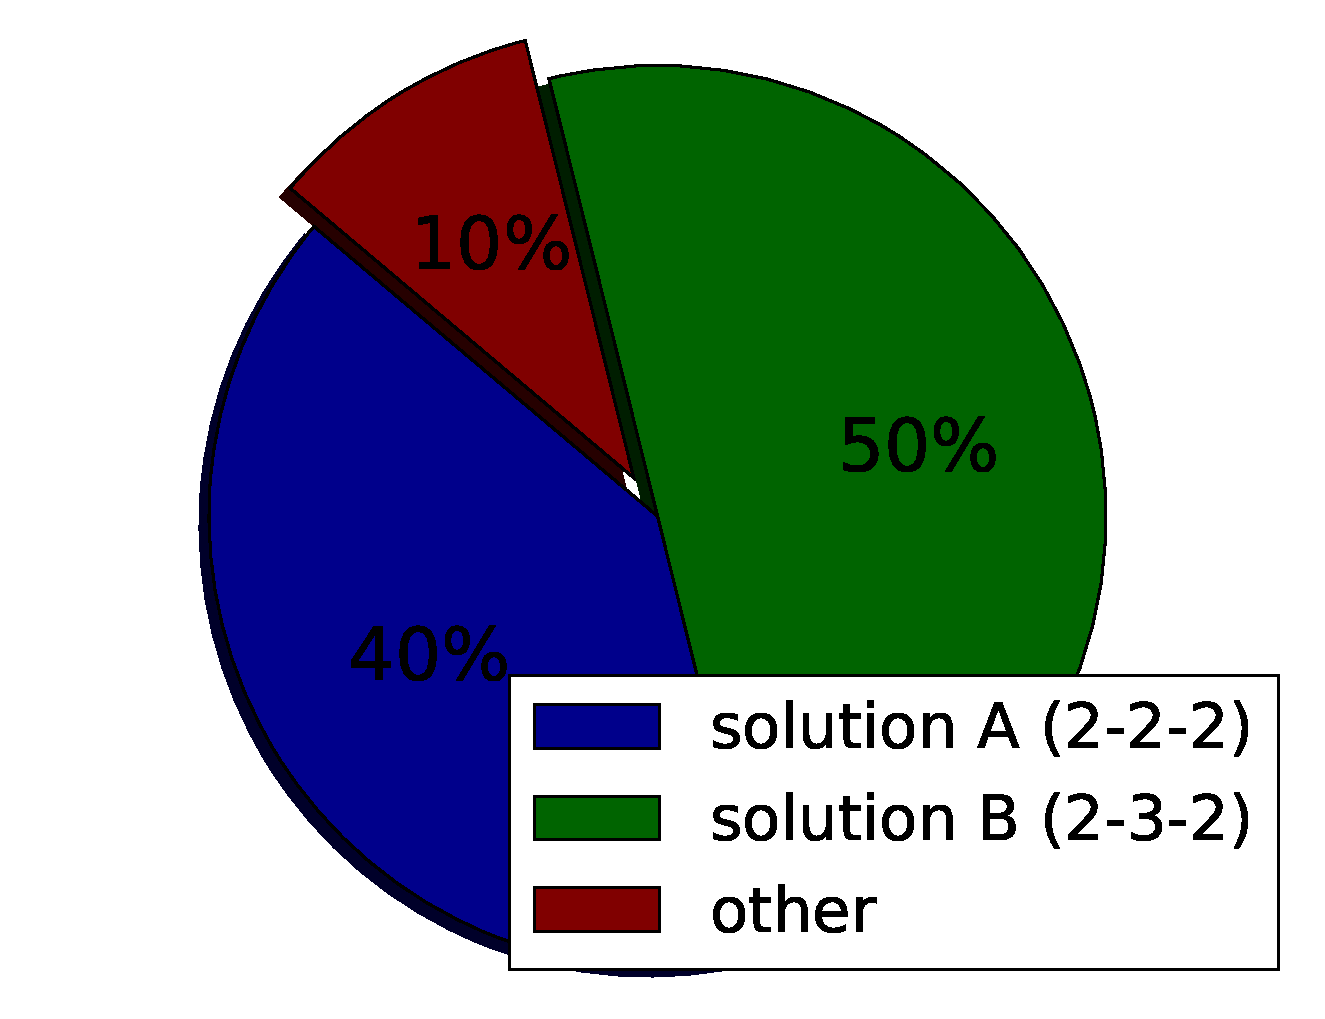
\includegraphics[height=4cm]{pruning_result_pie_xor.eps}
  \caption{Network structure after pruning (100 observations).}
  \label{fig:examples:pie_xor}
\end{subfigure}
\begin{subfigure}{.4\textwidth}
  \centering
  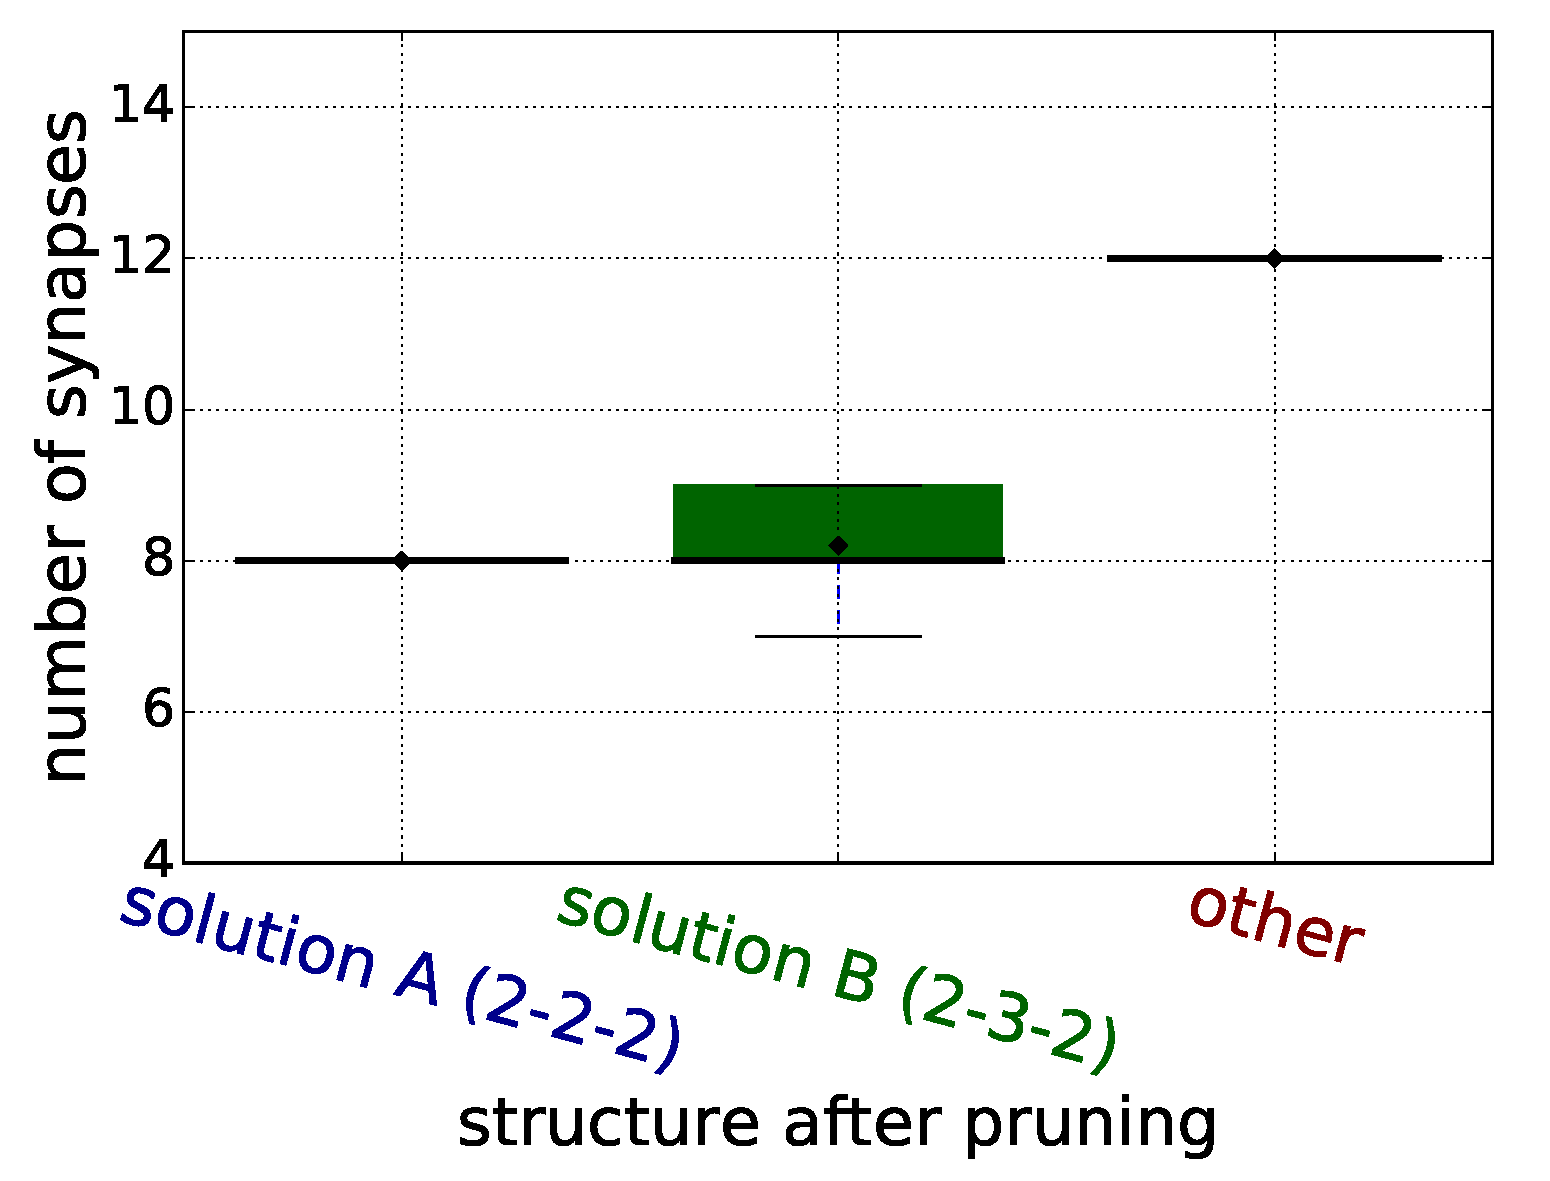
\includegraphics[height=4cm]{pruning_result_synapses_xor.eps}
  \caption{Number of synapses after pruning (100 observations).}
  \label{fig:examples:result_synapses_xor}
\end{subfigure}
\caption{Pruning results for XOR dataset.}
\label{fig:examples:pruning_result_xor}
\end{figure}

\section{2D-problem B: Unbalanced Features} \label{sec:dataset_unbfea}
This example is adopted from \citep{karnin}. The problem is again two-dimensional having two non-overlapping classes as depicted in \cref{fig:examples:dataset_unbfea}. The samples are uniformly distributed in $ [-1, 1] $ x $ [-1, 1] $ and the classes are equally probable, separated by two lines in 2D space ($ x_1 = a $ and $ x_2 = b $, where $ a = 0.1 $ and $ b = \frac{2}{a+1} - 1 $). Therefore, the problem can be solved by two neurons, similarly as the previous one.

What is interesting about this two-classes layout is that feature $ x_1 $ is much more important for the global classification accuracy than feature $ x_2 $. Having $ x_1 $ information, based on \cref{fig:examples:dataset_unbfea} one could potentially classify about $ 80-90\% $ of the samples. Opposite of that, we cannot say much with information from feature $ x_2 $ only. And this is something what also the pruning algorithm should find out.

\begin{figure}[H]
\centering
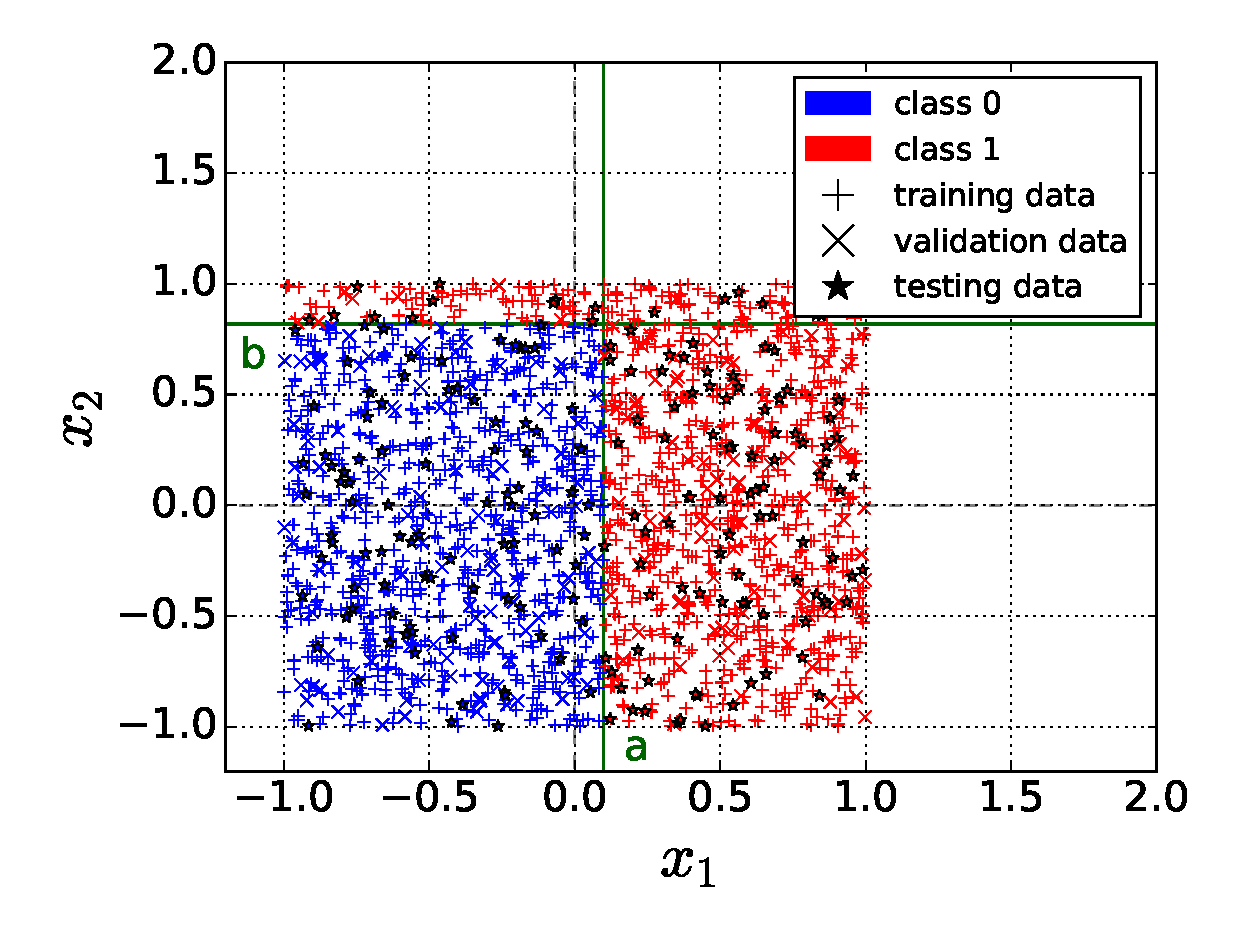
\includegraphics[width=\textwidth]{dataset_unbfea.eps}
\caption{A dataset with unbalanced feature importance.}
\label{fig:examples:dataset_unbfea}
\end{figure}

\subsection*{Results: Unbalanced Features}

\section{The Rule-plus-Exception Problem} \label{sec:dataset_rpe}
This problem is originally adopted from \citep{mozer_smolensky} and is also used in \citep{karnin}. The task is to learn another Boolean function: $ AB+\overline{ABCD} $. In this case the problem is four-dimensional. A single function output should be on (i.e. equals 1) when both $ A $ and $ B $ are on, which is the \textit{rule}. It should also be on when the \textit{exception} $ \overline{ABCD} $ occurs.

Clearly, the \textit{rule} occurs more often than the \textit{exception}, therefore the samples corresponding with the \textit{rule} should be more important for the global classification accuracy. The hypothesis is that the pruning method will reveal the part of network, which deals with the \textit{exception}, to be eliminated first - before the part of network dealing with the \textit{rule}.

\subsection*{Results: The Rule-plus-Exception}

\section{The Train Problem} \label{sec:dataset_train}
The Michalski's train problem...

\begin{figure}[H]
\centering
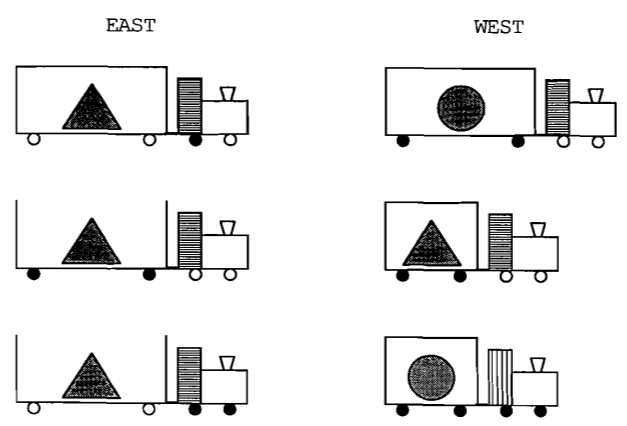
\includegraphics[width=\textwidth]{train_problem}
\caption{Michalski's train problem.}
\label{fig:examples:dataset_train}
\end{figure}

\section{Handwritten digits (MNIST)} \label{sec:dataset_mnist}
MNIST data... \citep{online:mnist}

\section{Phonemes (Speech Data)} \label{sec:dataset_phonemes}
PHONES data...
